\documentclass[letterpaper,12pt]{article}
\usepackage{mathtools}
\DeclarePairedDelimiter\abs{\lvert}{\rvert}     %serve per mettere il modulo 
\usepackage{booktabs}
\usepackage{bm}
\usepackage{colortbl}
\usepackage{tabularx}
\usepackage{textcomp}
\usepackage{siunitx}
\usepackage{booktabs}
\usepackage{enumitem}
\usepackage{xcolor}
\usepackage{fancyhdr}
\usepackage{caption}
\usepackage{changepage}
\usepackage{amsmath} 
\usepackage{subcaption}
\usepackage{graphicx}
\usepackage[table]{xcolor} 
\usepackage[margin=1in,letterpaper]{geometry} % decreases margins
\usepackage{cite} % takes care of citations
\usepackage[hidelinks]{hyperref} % adds hyper links inside the generated pdf file
% Define the colors
\definecolor{linkcolor}{RGB}{0, 102, 204}
\definecolor{citecolor}{RGB}{34, 139, 34}
\definecolor{urlcolor}{RGB}{255, 69, 0}

% Setup hyperref
\hypersetup{
    colorlinks=false, % colored links
    linkcolor=linkcolor, % color for internal links
    citecolor=citecolor, % color for citations
    urlcolor=urlcolor, % color for URLs
}
\fancypagestyle{logoheader}{
    \fancyhf{}
    \fancyhead[L]{
\includegraphics[width = 3cm]{infn-art-science-universita-degli-studi-di-milano-bicocca-maintainer-universita-studi-milano-bicocca.png}}
    \renewcommand{\headrulewidth}{0pt}
    }
\usepackage{blindtext}
\graphicspath{{immagini/}}
%Required for inserting images
%++++++++++++++++++++++++++++++++++++++++
%Margini 



\begin{document}

\title{{\small Università degli studi Milano-Bicocca  Dipartimento di Fisica - Laboratorio II }\\
	Esperienza Ottica - Microonde}
\author{F. Ballo, S. Franceschina, S. Dolci - Gruppo T1 39}
\date{\today}
\maketitle
\thispagestyle{logoheader}


\begin{abstract}
	Nella seguente relazione vengono presentati i risultati ottenuti dalla quarta esperienza del corso di Laboratorio II riguardante l'analisi di fenomeni ottici. L'obiettivo di questa esperienza è quello di studiare le proprietà caratteristiche delle onde elettromagnetiche nello spettro delle microonde. Ci si rifà all'utilizzo di emettitori e ricevitori per registrare il segnale delle onde altrimenti invisibili all'occhio umano (lunghezza d'onda circa 2.85cm).
	\begin{adjustwidth}{-1cm}{-1cm}
	\end{adjustwidth}
\end{abstract}
\tableofcontents
\newpage

\section{Caratteristiche del fascio}

\subsection{Configurazione del circuito e della strumentazione}
Di seguito riportiamo informazioni sulla strumentazione e sulle modalità di misura

\subsection{Polarizzazione}

Il primo obbiettivo dell'esperienza è stato quello di caratterizzare il fascio di microonde emesso dall'emettitore.
Per fare ciò, abbiamo cominciato verificando la direzione di polarizzazione del fascio. \\
Abbiamo posizionato l'emettitore e il ricevitore uno di fronte all'altro, in modo che fossero
allineati ed a una distanza fissa. Abbiamo quindi ruotato gradualmente il ricevitore e campionato
la tensione rilevata dal ricevitore, fino ad aver compiuto una rotazione di 180 gradi.\\
Dal manuale Pasco sappiamo che l'emettitore emette un fascio coerente polarizzato linearmente
e il ricevitore è sensibile solo ad una certa polarizzazione. Il comportamento che ci aspettiamo
di osservare da questo esperimento è quello previsto dalla legge di Malus:
\begin{equation}
	I = I_0 \cos^2(\theta)
	\label{eq:malus}
\end{equation}
Dove $I_0$ è l'intensità massima e $\theta$ è l'angolo tra la direzione di polarizzazione del fascio e quella rilevata dal ricevitore.\\

\begin{figure}[h!]
	\centering
	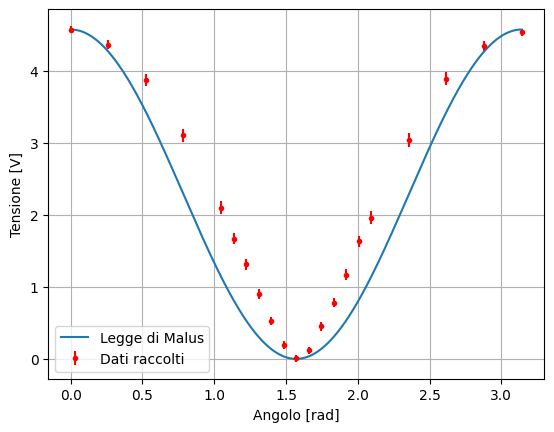
\includegraphics[width = 0.7\textwidth]{polarizzazione.png}
	\caption{Intensità del segnale rilevato in funzione dell'angolo di rotazione}
	\label{fig:polarizzazione}
\end{figure}
\paragraph*{Finire la conclusione e manca la parte del filtro polarizzatore}

\subsection{Ampiezza}
\subsubsection{Intensità in funzione dell'angolo di rotazione}

\begin{figure}[h!]
    \centering
    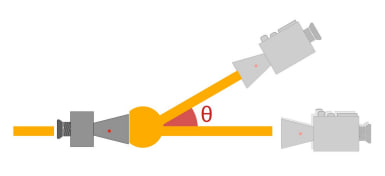
\includegraphics[width = 0.4\textwidth]{ampiezza rotazione.jpg}
    \caption{Impostazione dell'apparato per la misura dell'ampiezza del segnale in funzione dell'angolo di rotazione}
    \label{fig:ampiezza_angolo}
\end{figure}

Dopo aver concluso che il rilevatore reagisce all'intensità del segnale, ci siamo dedicati allo studio della geometria
del fascio emesso. Per prima cosa, abbiamo studiato la variazione dell'intensità rilevata al variare dell'angolo di rotazione
tra emettitore e ricevitore.\\
Per fare ciò, abbiamo fissato una distanza tra i due dispositivi e ruotato gradualmente il ricevitore attorno ad un asse
passante di fronte all'emettitore. Abbiamo poi campionato la tensione rilevata dal ricevitore ad intervalli di 5 gradi, fino a quando
il valore misurato è calato a circa zero.\\
Di seguito riportiamo i dati raccolti:

\begin{figure}[h!]
    \centering
    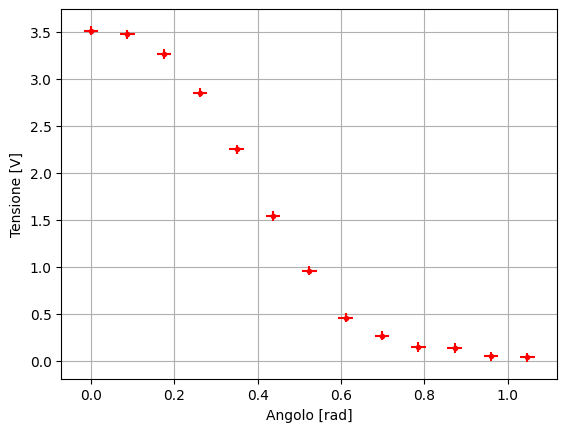
\includegraphics[width = 0.6\textwidth]{dati_rotazione.png}
    \caption{Intensità del segnale rilevato in funzione dell'angolo di rotazione}
    \label{fig:rotazione}
\end{figure}

Per stabilire quale modello stessero seguendo i dati, abbiamo scelto di interpolarli prima con una funzione coseno generica,
successivamente con una funzione coseno elevato ad una potenza ignota:
\begin{align}
    & I = A\cos(Bx + C) + D \\
    & I = A\cos^(Bx + C) + D
\end{align} 

\subsubsection{Intensità in funzione della distanza}

\begin{figure}[h!]
    \centering
    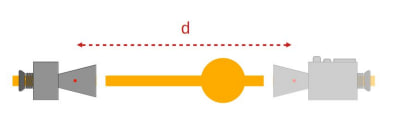
\includegraphics[width = 0.45\textwidth]{ampiezza distanza.jpg}
    \caption{Impostazione dell'apparato per la misura dell'ampiezza del segnale in funzione della distanza tra emettitore e ricevitore}
    \label{fig:ampiezza_distanza}
\end{figure}

Il punto successivo consisteva nello studiare l'andamento dell'intensità del segnale in funzione della distanza tra i
dispositivi. Mantenendo l'emettitore e il ricevitore allineati, abbiamo variato la separazione tra i due
e campionato a intervalli regolari la tensione misurata.\\
A causa del fatto che emettitore e ricevitore si trovavano uno di fronte all'altro, oltre alla decrescita
del segnale dovuta alla distanza, abbiamo osservato un andamento oscillatorio. Questo è dovuto al fatto che
parte del segnale inviato non viene assorbita dal rilevatore, ma viene riflessa e ritorna verso l'emettitore,
che a sua volta riflette parte del segnale. Si forma quindi un'onda stazionaria tra i due dispositivi,
la cui interferenza porta a un andamento oscillatorio dell'intensità osservata.\\
Per cominciare abbiamo campionato ogni 1 cm, per analizzare l'andamento generale del fascio; successivamente,
ci siamo ristretti attorno ad alcuni massimi e misurato con passi di 0.2 cm per farci un idea migliore della lunghezza d'onda.\\

\begin{figure}[h!]
	\centering
	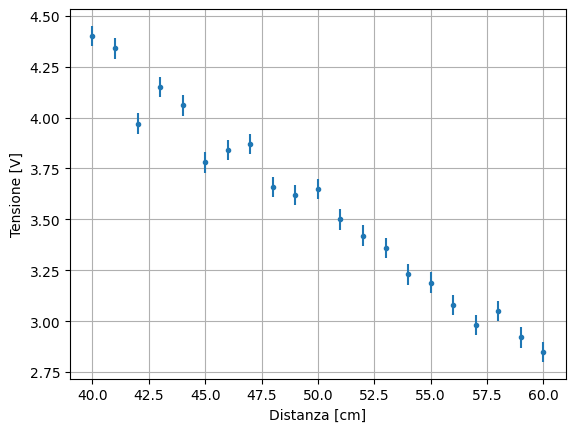
\includegraphics[width = 0.6\textwidth]{dati_distanza.png}
	\caption{Intensità del segnale rilevato in funzione della distanza}
	\label{fig:distanza}
\end{figure}

\paragraph*{Andamento globale del segnale}
Se il fascio si comportasse come un'onda piana ideale, ci aspetteremmo che la sua intensità non dipendesse dalla distanza.
Se invece si comportasse come un'onda sferica, l'andamento dell'intensità dovrebbe essere inversamente proporzionale
al quadrato della distanza. Nella realtà, il segnale avrà un andamento più complesso che non si adatterà perfettamente
a nessuna delle due funzioni.\\
Per capire quale fosse l'andamento dell'intensità del segnale, abbiamo deciso di interpolare i dati con diverse funzioni,
per vedere quale fosse la più adatta.\\

\begin{figure}[h!]
	\centering
	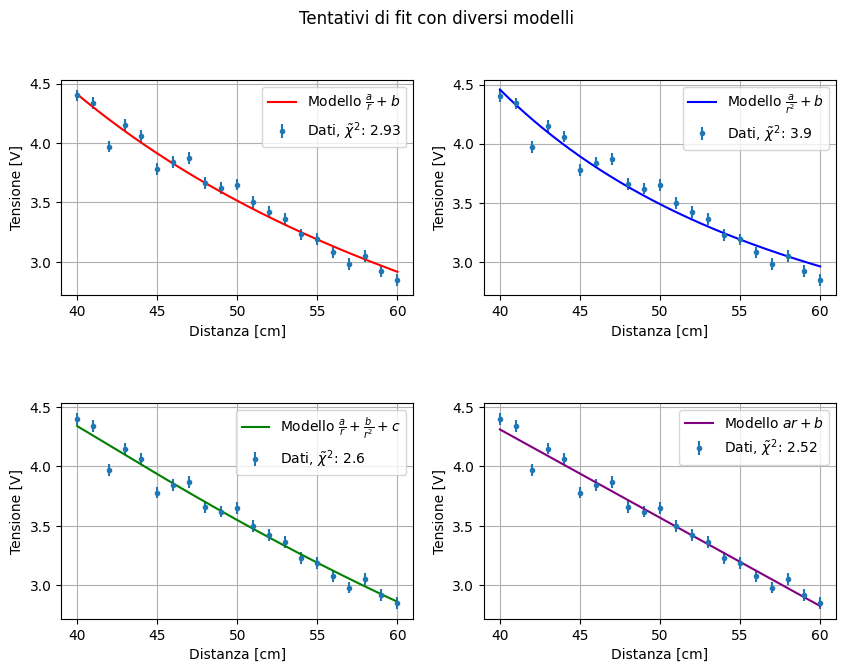
\includegraphics[width = \textwidth]{fit_distanza_vari_modelli.png}
	\caption{Fit dell'intensità del segnale rilevato in funzione della distanza secondo diversi modelli}
	\label{fig:fit_distanza_vari_modelli}
\end{figure}

Non avendo una risoluzione sufficiente per distinguere con precisione massimi e minimi, abbiamo deciso di interpolare
i dati con funzioni non oscillanti. Per giustificare questa scelta, abbiamo considerato che le oscillazioni dovute all'interferenza
variano attorno ad un valore medio, e che i contributi dovuti ad ogni particolare oscillazione in media si annullano a vicenda.\\
Osservando i grafici in figura \ref{fig:fit_distanza_vari_modelli}, si evince che tra quelli considerati, il modello che meglio si adatta
ai dati è lineare.

\newpage
\paragraph*{Andamento attorno ai massimi}
Successivamente, abbiamo proceduto ricavando la lunghezza d'onda del fascio dai dati campionati più frequentemente, riportati nella figura di seguito.

\begin{figure}[h!]
	\centering
	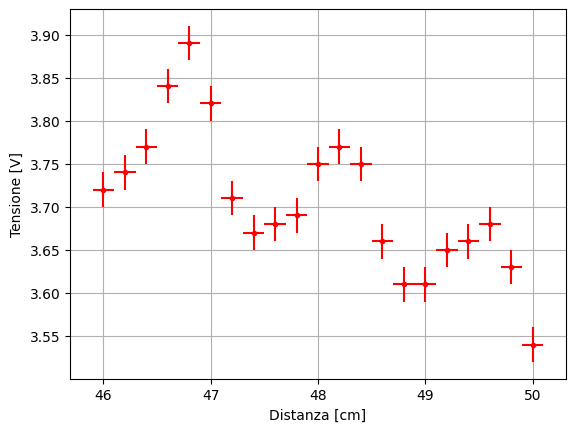
\includegraphics[width = 0.7\textwidth]{dati_distanza_ondulatori.png}
	\caption{Intensità del segnale rilevato in funzione della distanza - zoom attorno ad alcuni massimi}
	\label{fig:distanza_zoom}
\end{figure}

Avendo stabilito che l'andamento dell'intensità del segnale era lineare, abbiamo deciso di interpolare i dati con una funzione del tipo:
\begin{equation}
	I = Ax + B\ + Csin(Dx + E)
	\label{eq:modello_oscillante}
\end{equation}
che corrisponde ad una retta con un'onda sinusoidale sovrapposta.\\
Il risultato del fit è riportato in figura \ref{fig:fit_distanza_ondulatori}.

\begin{figure}[h!]
	\centering
	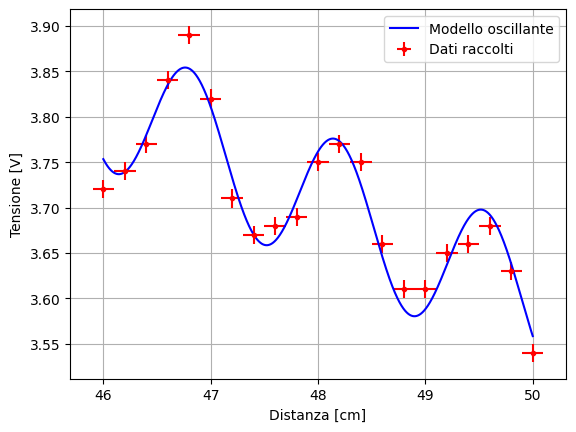
\includegraphics[width = 0.7\textwidth]{fit_distanza_ondulatori.png}
	\caption{Fit dell'intensità del segnale rilevato in funzione della distanza campionato più frequentemente}
	\label{fig:fit_distanza_ondulatori}
\end{figure}

Il fit ha restituito i seguenti valori: (magari una tabella esce meglio)
\begin{enumerate}
	\item $A = -0.057 \pm 0.004$
	\item $B = 6.43 \pm 0.18$
	\item $C = 0.077 \pm 0.006$
	\item $D = 4.56 \pm 0.06$
	\item $E = -67.5 \pm 3.1$
	\item $\tilde\chi^2 = 1.1$
\end{enumerate}

In questo caso il valore $D$ rappresenta il numero d'onda, quindi la lunghezza d'onda è data da
$$\lambda = 2\cdot \frac{2\pi}{D}$$
dove il fattore 2 sta ad indicare il fatto che la lunghezza d'onda del fascio emesso è il doppio della lunghezza d'onda del segnale che interferisce.\\
Inserendo i valori ottenuti dal fit, propagando l'errore ed eseguendo un test di compatibilità, otteniamo:
\begin{align*}
	 & \lambda = (2.75 \pm 0.04)\ \text{m} \\
	 & \text{compatibilità}: 2.47
\end{align*}

\subsection{Conclusioni}

\section{Angolo di Brewster}
In questa sezione abbiamo studiato il raggio trasmesso e riflesso da una lastra di polietilene al fine di determinare
l'angolo di Brewster.\\
Per l'analisi del raggio trasmesso abbiamo posto il ricevitore di fronte al trasmettitore, frapponendo la lastra
fra i due. Abbiamo montato la lastra su un supporto rotante e e variando in tal modo l'angolo di incidenza del raggio
abbiamo campionato l'intensità del raggio trasmesso.\\
Per verificare il fatto che l'intensità del raggio trasmesso sia dipendente anche dalla polarizzazione abbiamo
eseguito la stessa procedura per due differenti polarizzazioni, rouotando l'emettitrore di 90 gradi. Per la polarizzazione
parallela alla lastra, al fine di trovare l'angolo di Brewster, abbiamo interpolato il picco con un modello parabolico,
che riportiamo:
\begin{equation}
	y = a(x-b)^2 + c
	\label{eq:parabola}
\end{equation}
\\

Per l'analisi del raggio riflesso abbiamo configurato l'apparato in modo tale da far variare sia l'angolo della lastra,
sia l'angolo tra emettitore e ricevitore, in modo che il ricevitore seguisse il raggio riflesso. Abbiamo così campionato
l'intensità del raggio riflesso al variare dell'angolo di incidenza.\\

\subsection{Analisi dati}

Riportiamo di seguito il grafico dell'intensità del raggio trasmesso in funzione dell'angolo di incidenza.\\
\begin{figure}[h!]
	\centering
	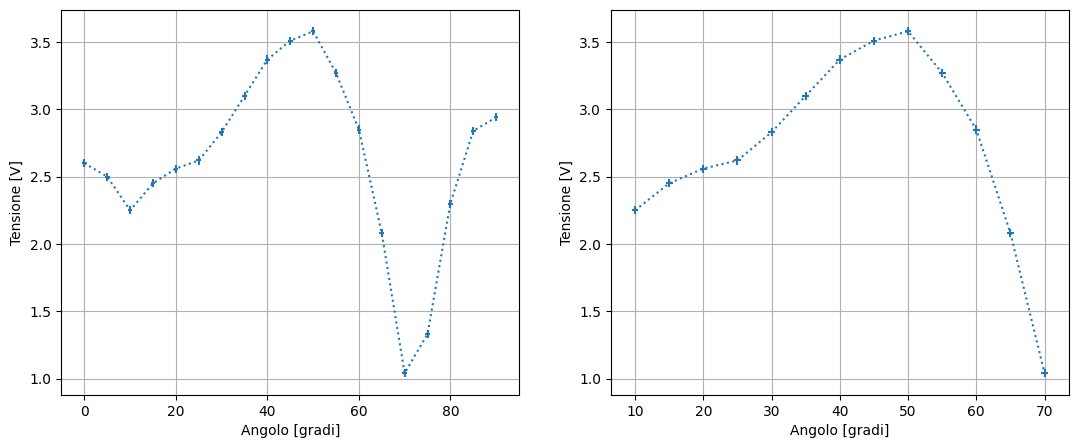
\includegraphics[width = 0.8\textwidth]{trasmesso.png}
	\caption{Intensità del raggio trasmesso in funzione dell'angolo di incidenza}
	\label{fig:trasmesso}
\end{figure}

Abbiamo inserito il grafico con tutte le misurazioni effettuate (grafico di sinistra). Analizzando la figura ci
siamo accorti che l'intensità torna ad aumentare oltre 70 gradi. Questo è dovuto al fatto che la lastra, non essendo
abbastanza lunga, lasciava passare parte del raggio incidente, determinando un aumento dell'intensità. Abbiamo quindi
deciso di escludere gli ultimi dati poichè non rilevanti per il fenomeno. Vengono riportati nel grafico di destra
i valori che abbiamo utilizzato per l'analisi.\\
Una volta individuata la regione in cui l'intensità aumentava, abbiamo interpolato il picco con un modello parabolico.
Vengono riportate l'interpolazione, i parametri ottenuti e il valore di $\chi^2$:

\begin{figure}[h!]
	\centering
	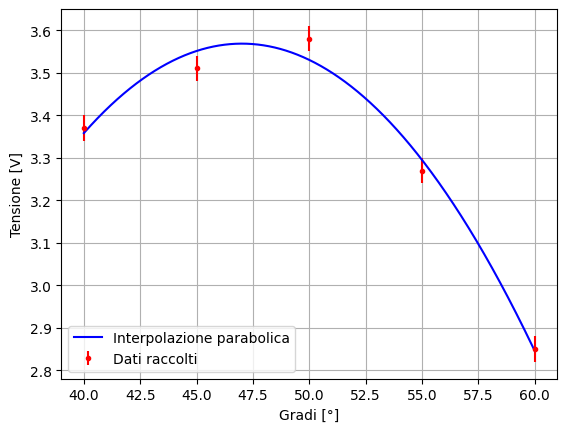
\includegraphics[width = 0.8\textwidth]{brew_angle.png}
	\caption{Interpolazione del picco con modello parabolico}
	\label{fig:parabola}
\end{figure}

%Da cambiare i valori con quelli ottenuti dal fit (manca la propagazione degli errori x2y)
\begin{enumerate}
	\item $a = 0.0003 \pm 0.0001$
	\item $b = 0.0003 \pm 0.0001$
	\item $c = 0.0003 \pm 0.0001$
	\item $\chi^2 = 0.0003$
\end{enumerate}

Il parametro b, essendo la traslazione della parabola sull'asse x, rappresenta l'angolo di Brewster. Abbiamo
confrontato l'angolo ottenuto con l'angolo atteso, ottenendo una distanza in deviazioni standard di: DA INSERIRE\\

Riportiamo in figura \ref{fig:wrong_pol} il grafico dell'intensità del raggio trasmesso per la polarizzazione
perpendicolare alla lastra. Abbiamo escluso le ultime misure per lo stesso motivo dell'analisi di raggio trasmesso
con polarizzazione parallela.\\

\begin{figure}[h!]
	\centering
	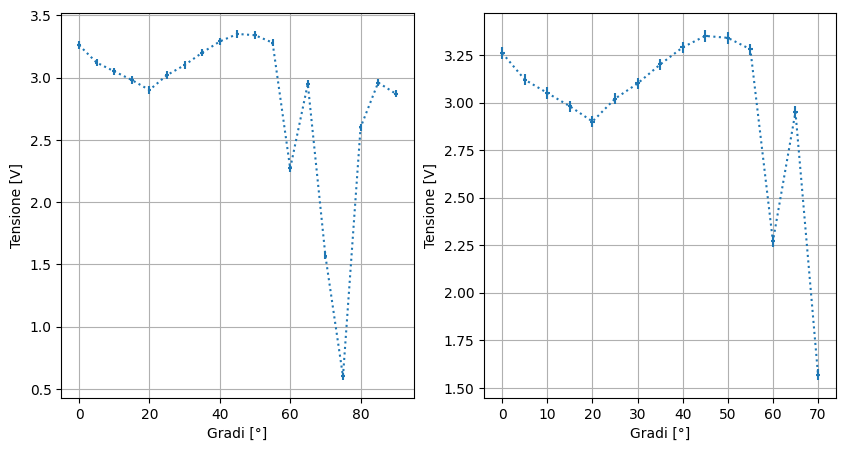
\includegraphics[width = 0.8\textwidth]{wrong_pol.png}
	\caption{Intensità del raggio trasmesso - polarizzazione perpendicolare}
	\label{fig:wrong_pol}
\end{figure}

Per quanto riguarda i dati e i grafici relativi all'intensità del raggio riflesso, li riportiamo per completezza,
nonostante siano intrattabili dal punto di vista dell'analisi. Avendo osservato ciò già nella prima giornata di
laboratorio, abbiamo effettuato nuovamente le stesse misure nella seconda giornata, ma senza ottenere miglioramenti.
L'andamento globale dei grafici richiama quello corretto, ma i numerosi picchi fanno intuire la necessità di un
campionamento maggiore, come spiegato nelle conclusioni.\\

\begin{figure}[h!]
	\centering
	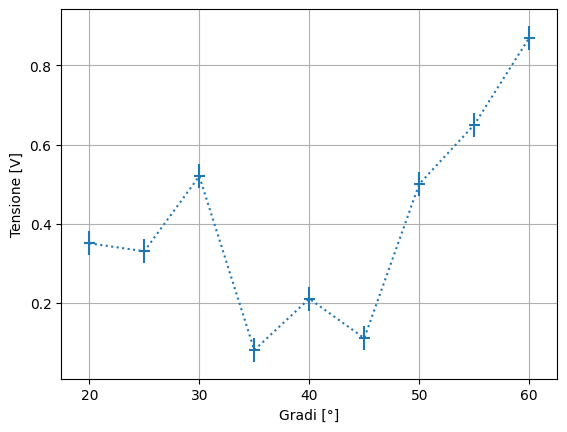
\includegraphics[width = 0.8\textwidth]{riflesso1.png}
	\caption{Intensità del raggio riflesso - prima giornata}
	\label{fig:riflesso1}
\end{figure}

\begin{figure}[h!]
	\centering
	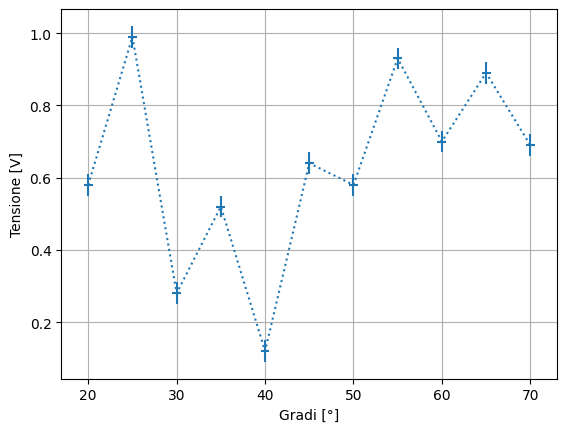
\includegraphics[width = 0.8\textwidth]{riflesso2.png}
	\caption{Intensità del raggio riflesso - seconda giornata}
	\label{fig:riflesso2}
\end{figure}

\subsection{Conclusioni}

\section{Interferenza}
Per la sezione di interferenza abbiamo scelto l'interferometro di Lloyd e l'interferometro di Michelson.\\

\subsection{Specchio Lloyd}
In questa sezione abbiamo utilizzato uno specchio di Lloyd per osservare l'interferenza tra i due fasci di microonde.
Abbiamo disposto emettitore e ricevitore uno di fronte all'altro, misurandone la distanza $d$, in seguito abbiamo
posizionato una lastra riflettente ad una certa distanza $h$ dal centro. \\
In questo modo si vengono a creare due fasci: il primo percorre una distanza $d$ in linea retta, mentre il secondo
percorre una distanza $2\ \sqrt[]{h^2 + (d/2)^2}$. Tale differenza di percorso porta a delle interferenze:
se la differenza di cammino ottico è un multiplo intero di $\lambda$ si ha interferenza costruttiva,
altrimenti si ha interferenza distruttiva.\\
Al fine di misurare la lunghezza d'onda delle microonde, abbiamo seguito le istruzioni fornite dal manuale
PASCO e abbiamo variato la distanza $h$ alla ricerca di due minimi distanti dieci volte la lunghezza d'onda,
una volta fissata la distanza $d$. Per poter eseguire un confronto sperimentale e non solo con il valore di $\lambda$
tabulato, abbiamo ripetuto la procedura per un'altra distanza $d$. \\
Come formula per il calcolo della lunghezza d'onda abbiamo utilizzato la seguente, ricavata dalle relazioni geometriche
che legano i cammini ottici e la differenza di fase tra i due fasci:
\begin{equation}
	\lambda = \frac{2h + 4\ \sqrt[]{(d/2)^2 + h^2}}{n}
	\label{eq:lloyd}
\end{equation}
Dalla prima misurazione abbiamo ottenuto due valori di $\lambda$ che abbiamo mediato, lo stesso abbiamo fatto per
la seconda misurazione.Come errori delle singole lunghezze d'onda abbiamo propagato gli errori a partire dall'equazione
\ref{eq:lloyd}, in seguito abbiamo propagato gli errori per la media. \\


\subsubsection{Analisi dati}
Riportiamo di seguito i dati raccolti durante l'esperienza e i risultati ottenuti.
Per la prima misurazione abbiamo scelto $d = 100 \pm 1$ cm, mentre per la seconda $d = 110 \pm 1$ cm. Abbiamo stimato
le incertezze di 1 cm poichè sugli "horn" non erano ben segnalati i punti di emissione e di ricezione
dell'onda; non sapendo bene dove fossero localizzati abbiamo aumentato l'errore rispetto alla sensibilità della riga
graduata.\\
In tabella \ref{tab:lloyd1} riportiamo i valori di $h$ e le intensità misurate per i minimi di interferenza,
in tabella \ref{tab:lloyd2} riportiamo i valori di $h$ e le intensità misurate per i massimi di interferenza.\\
Come valore $\lambda_1$ abbiamo ottenuto $2.86 \pm 0.07$ cm, mentre per $\lambda_2$ abbiamo ottenuto $2.85 \pm 0.06$ cm.\\
Abbiamo confrontato i valori ottenuti con il valore tabulato di $\lambda = 2.85$ cm, ottenendo:
\begin{enumerate}
	\item Distanza in deviazioni standard tra $\lambda_1$ e $\lambda_{tab}$: $0.11 \sigma$
	\item Distanza in deviazioni standard tra $\lambda_2$ e $\lambda_{tab}$: $0.08 \sigma$
	\item Distanza in deviazioni standard tra $\lambda_1$ e $\lambda_2$: $0.03 \sigma$
\end{enumerate}
L'ultimo punto è stato calcolato per verificare la coerenza tra i due valori di $\lambda$ ottenuti.\\

\subsubsection{Conclusioni}
Dai risultati ottenuti possiamo concludere che la lunghezza d'onda delle microonde calcolata tramite interferometro
di Lloyd è compatibile con il valore tabulato.
Al di là della misura della lunghezza d'onda tramite interferenza, questa sezione ci ha permesso di verificare
sperimentalmente un'ipotesi che avanziamo in altre sezioni: l'interferenza per riflessione delle microonde. Ogniqualvolta
un esperimento richieda la rotazione del ricevitore, si possono considerare effetti di interferenza alla Lloyd,
poichè, per angoli in cui ricevitore e emettitore sono sempre più vicini, si può modelizzare il sistema come
un interferometro di Lloyd.\\
In conclusione, l'interferenza alla Lloyd si ottiene quando un materiale che abbia proprietà riflettenti viene
avvicinato all'apparecchiatura, portandoci a considerare questo effetto di interferenza in tutte le sezioni in cui
ci troviamo a ruotare il ricevitore.\\


\subsection{Interferometro di Michelson}


\subsubsection{Analisi Dati Michelson}


\section{Diffrazione di Bragg}

\subsection{Analisi Dati Bragg}

\newpage
\section{Tabelle misurazioni}

\begin{table}[h!]
	\centering
	\caption{Lloyd: prima misura}
	\label{tab:lloyd1}
	\begin{tabular}{|c|c|}
		\hline
		$h$ [cm] & $I$ [V] \\
		\hline
		9.9      & 1.64    \\
		16.9     & 1.7     \\
		\hline
	\end{tabular}
\end{table}

\begin{table}[h!]
	\centering
	\caption{Lloyd: seconda misura}
	\label{tab:lloyd2}
	\begin{tabular}{|c|c|}
		\hline
		$h$ [cm] & $I$ [V] \\
		\hline
		10.9     & 1.40    \\
		17.2     & 1.5     \\
		\hline
	\end{tabular}
\end{table}

10.9
v4 = 1.40
h4 = 17.2
v4 = 1.5

\end{document}
